\documentclass[drones,article,submit,pdftex,moreauthors]{Definitions/mdpi}

\firstpage{1}
\makeatletter
\setcounter{page}{\@firstpage}
\makeatother
\pubvolume{1}
\issuenum{1}
\articlenumber{0}
\pubyear{2026}
\copyrightyear{2026}
\datereceived{}
\daterevised{}
\dateaccepted{}
\datepublished{}

\setlength{\headheight}{18.5pt}
\providecommand{\tightlist}{%
	\setlength{\itemsep}{0pt}\setlength{\parskip}{0pt}}

\Title{SentAI: An Open-Source Dual-Camera Edge AI Runtime for Vision-Guided Drone Autonomy on Coral Micro}

\Author{Author Name $^{1,}$*}
\AuthorNames{Author Name}

\address{$^{1}$ \quad Affiliation, City, Country; email@example.com}

\corres{Correspondence: email@example.com}

\abstract{This paper presents SentAI, an open-source MicroPython environment for high-level autonomous flight control on a minimalist embedded AI board that integrates an EdgeTPU accelerator and extends it with two 5 Mpx cameras and an onboard IMU. The platform is designed as a compact sensing and decision layer for micro-aerial vehicles, combining scriptable mission logic, dynamic TensorFlow Lite model loading, continuous onboard inference, and real-time communication in a resource-constrained MCU system. The work explicitly targets two complementary UAV workflows: Bitcraze Crazyflie for agile indoor experimentation and PX4/MAVLink-oriented autopilot integration for more transferable field deployment. At the perception level, SentAI provides a dual-camera, multi-model runtime with camera switching, per-camera geometry, lightweight tracking, motion compensation, and ground-aware spatial reasoning. A central contribution is the systems-level engineering of the complete visual path from sensor capture to EdgeTPU input, including DMA-backed acquisition, hardware-assisted image preparation, memory placement across internal RAM and SDRAM, and pipelined FreeRTOS scheduling that overlaps capture, preprocessing, and inference. The implementation therefore treats throughput, buffer ownership, and accelerator feeding as first-class design constraints rather than secondary optimization details. Beyond the runtime itself, the work is framed by an open synthetic dataset and a custom YOLO model intended for low-altitude drone navigation in inhabited environments. The result is an embedded autonomy stack that moves an open-source prototype platform toward a more industrialized, production-oriented runtime for lightweight drone research and deployment.}

\keyword{embedded AI; EdgeTPU; MicroPython; drone autonomy; Coral Micro; MAVLink; Crazyflie; dual camera; FreeRTOS}

\addhighlights{yes}
\renewcommand{\addhighlights}{%
\noindent\textbf{What are the main findings?}
\begin{itemize}[labelsep=2.5mm,topsep=2pt]
\item SentAI turns Coral Micro into a dual-camera embedded autonomy runtime for drones with MicroPython control and onboard EdgeTPU inference.
\item The implementation shows that throughput on a compact MCU-plus-accelerator platform depends critically on RTOS scheduling, memory placement, and hardware-assisted image preparation.
\end{itemize}
\textbf{What are the implications of the main findings?}
\begin{itemize}[labelsep=2.5mm,topsep=2pt]
\item Lightweight UAV platforms can support richer onboard perception when sensing, memory, and accelerator feeding are co-designed rather than treated as separate problems.
\item An open-source board can be pushed from proof-of-concept status toward a more production-oriented embedded AI stack suitable for repeatable autonomy experiments.
\end{itemize}
}

\begin{document}

\section{Introduction}
Autonomous visual navigation for small drones sits at the intersection
of several conflicting constraints: low mass, low power, real-time
perception, onboard decision making, and enough software flexibility to
support rapid iteration. In practice, many platforms solve only part of
this problem. Very small aerial vehicles are easy to fly indoors and
safe to test in tight environments, but they often lack the compute and
memory budget required by modern object detection pipelines. At the
opposite end, larger embedded AI platforms such as Coral Dev Board or
NVIDIA Jetson-class systems provide significantly more resources, but
they also bring higher current consumption, larger batteries, more
weight, and a form factor that is difficult to justify for lightweight
micro-UAV missions.

This work starts from an open-source platform with clear latent
potential, namely Coral Micro, and treats it not as a finished product
but as a promising technical base that can be pushed toward a much
higher level of systems maturity. The research direction is therefore
not limited to adding isolated features. Instead, it aims to move an
accessible open hardware and open software project toward an
industrialized embedded-AI stack with production-oriented performance
characteristics, stronger runtime guarantees, richer sensing, and a more
coherent control and telemetry model.

The starting point of this work was the need for a platform that remains
physically lightweight and energy-efficient, while still exploiting as
much as possible the inference capability of the EdgeTPU and the
real-time performance of the MCU. The original minimalist EdgeTPU-based
board configuration was attractive from the perspective of size and
power, but its standard low-resolution camera workflow was not
sufficient for the class of missions targeted here. In particular, a
320x240 sensing regime is too restrictive when the goal is to support
richer object detection, stricter scene understanding, and
higher-confidence flight decisions in inhabited or cluttered spaces.
This became even more limiting when considering modern YOLO-style
detectors, which benefit from larger spatial inputs and from a sensor
pipeline capable of preserving more detail before resizing and
quantization.

The objective of SentAI is therefore to define a new point in the design
space: a board-level and software-level architecture that preserves the
low-weight, low-power philosophy of minimalist embedded AI hardware, but
extends it toward practical autonomous drone operation. The platform
couples an MCU and an EdgeTPU with two 5 Mpx cameras and an onboard IMU,
and exposes the whole sensing, inference, communication, and control
stack through a MicroPython environment. This makes it possible to write
high-level mission logic in Python while keeping timing-critical
operations in the underlying real-time operating system and accelerator
path. The result is not only a development framework, but also a systems
study of how far one can push a compact embedded AI board toward real
airborne autonomy and toward a level of robustness closer to
production-grade embedded deployment.

The work explicitly targets two flight platforms. The first is Bitcraze
Crazyflie, used as an indoor experimental platform because it is agile,
lightweight, easy to maneuver, and well suited for repeated
safety-conscious testing in the laboratory. The second is a PX4-based
autopilot stack accessed through MAVLink, representing the path toward a
more professional and transferable deployment model. The intention is to
provide a common high-level autonomy layer across both targets, so that
mission scripts, perception logic, and communication flows can be
developed once and adapted across indoor research flights and more
operational MAVLink-centered scenarios.

From a vision-systems perspective, the work is driven by the observation
that model accuracy alone is not enough. Once YOLO-class detectors are
pushed toward larger inputs, for example 640-class or even workflows
derived from native 1280-wide camera imagery, the dominant issues become
memory layout, transfer scheduling, tensor preparation cost, and buffer
ownership between the camera subsystem, the MCU, and the EdgeTPU. For
this reason, the contribution is as much about systems engineering as it
is about AI. The implementation analyzes the full visual path from image
acquisition at the sensor, through DMA-backed capture into RAM, through
hardware pixel conversion and scaling, and finally into the EdgeTPU
input memory. These stages are pipelined in parallel under the RTOS so
that camera capture and image preparation can overlap with inference,
thereby maximizing frame rate while minimizing idle time and unnecessary
copies.

An important architectural extension is the addition of a dual-camera
subsystem. Instead of treating perception as a single fixed viewpoint
problem, SentAI supports two 5 Mpx sensors that may be mounted in
parallel or perpendicular configurations. This enables distinct
operational modes: forward-looking navigation together with nadir
inspection, redundant views for indoor localization, or viewpoint
switching according to the phase of the mission. The camera-switching
mechanism is designed as a first-class runtime concept, not as an
afterthought, and is supported by explicit per-camera geometry, frame
sequencing, and clean post-switch acquisition logic. Together with
IMU-aware tracking and ground-plane projection, this creates the basis
for drone-centric perception that is aware of mounting geometry and
flight context rather than only raw image content.

The work also extends beyond the runtime itself. In addition to dynamic
model loading and multi-model switching, the project assumes the
availability of a custom YOLO detector trained on an open synthetic
dataset built for low-altitude drone navigation in inhabited spaces. The
dataset contains views captured at nadir and at approximately 45
degrees, and is intended as a reusable pre-training or adaptation
resource for future systems that must obey stricter navigation and
avoidance logic in populated environments, including scenarios informed
by European drone categories such as A0-A3 and A2. This
dataset-and-model layer complements the embedded runtime by providing a
path from open training assets to open onboard deployment.

In this sense, the present work should be read as an industrialization
effort. Many of the underlying techniques are known in isolation:
embedded Python, edge inference, object detection, MAVLink
communication, or visual tracking. The novelty lies in bringing them
together on a highly constrained airborne computing platform and
resolving the practical bottlenecks that appear only during
implementation. These include memory fragmentation, RAM placement
between internal memory and external SDRAM, large tensor staging,
synchronization between RTOS tasks, camera switching latency, and the
challenge of sustaining high throughput without losing the low-power
character of the platform. The broader contribution is thus to
demonstrate how an open-source prototype platform can be evolved into a
system with much stronger production-oriented behavior, where
throughput, determinism, integration discipline, and operational
usability become design targets in their own right.

The main contributions of the work can be summarized as follows:

\begin{enumerate}
\def\labelenumi{\arabic{enumi}.}
\tightlist
\item
  An open-source MicroPython runtime for a lightweight EdgeTPU-enabled
  MCU platform intended for high-level autonomous drone control.
\item
  A dual-target flight-control concept spanning Bitcraze Crazyflie for
  indoor experimentation and PX4/MAVLink for professional autopilot
  integration.
\item
  A dual-camera 5 Mpx sensing architecture with onboard IMU support,
  runtime camera switching, per-camera geometry, and viewpoint-aware
  operation.
\item
  A real-time perception pipeline that studies and optimizes the
  end-to-end path from image sensor to MCU RAM to EdgeTPU memory, using
  parallel RTOS execution and double-buffered staging to maximize frame
  rate.
\item
  A memory-aware deployment strategy for YOLO-class detectors and other
  larger vision models on an MCU-constrained platform.
\item
  A multi-model workflow with dynamic model loading, context-dependent
  switching, tracking, projection to the ground plane, and telemetry
  integration.
\item
  An open synthetic aerial dataset and a custom YOLO model intended as a
  starting point for regulation-aware drone navigation in inhabited
  environments.
\end{enumerate}

The rest of the paper is organized as follows. The next section reviews
related work in autonomous nano-UAV navigation, embedded deep learning,
YOLO-based detection, MicroPython-enabled embedded control, and
accelerator-centric edge AI. The following sections present the hardware
and software architecture, the real-time memory and processing pipeline,
the communication and flight-control abstractions, and the experimental
perspective enabled by the platform.


\section{Related Work}
\input{paper_mdpi_related.tex}

\section{Materials and Methods}
\subsection{System Architecture and Design Rationale}
Figure~\ref{fig:impl01} summarizes the layered view of the platform, from sensing hardware and RTOS orchestration to EdgeTPU inference and the MicroPython experimentation surface.
\begin{figure}[H]
\centering
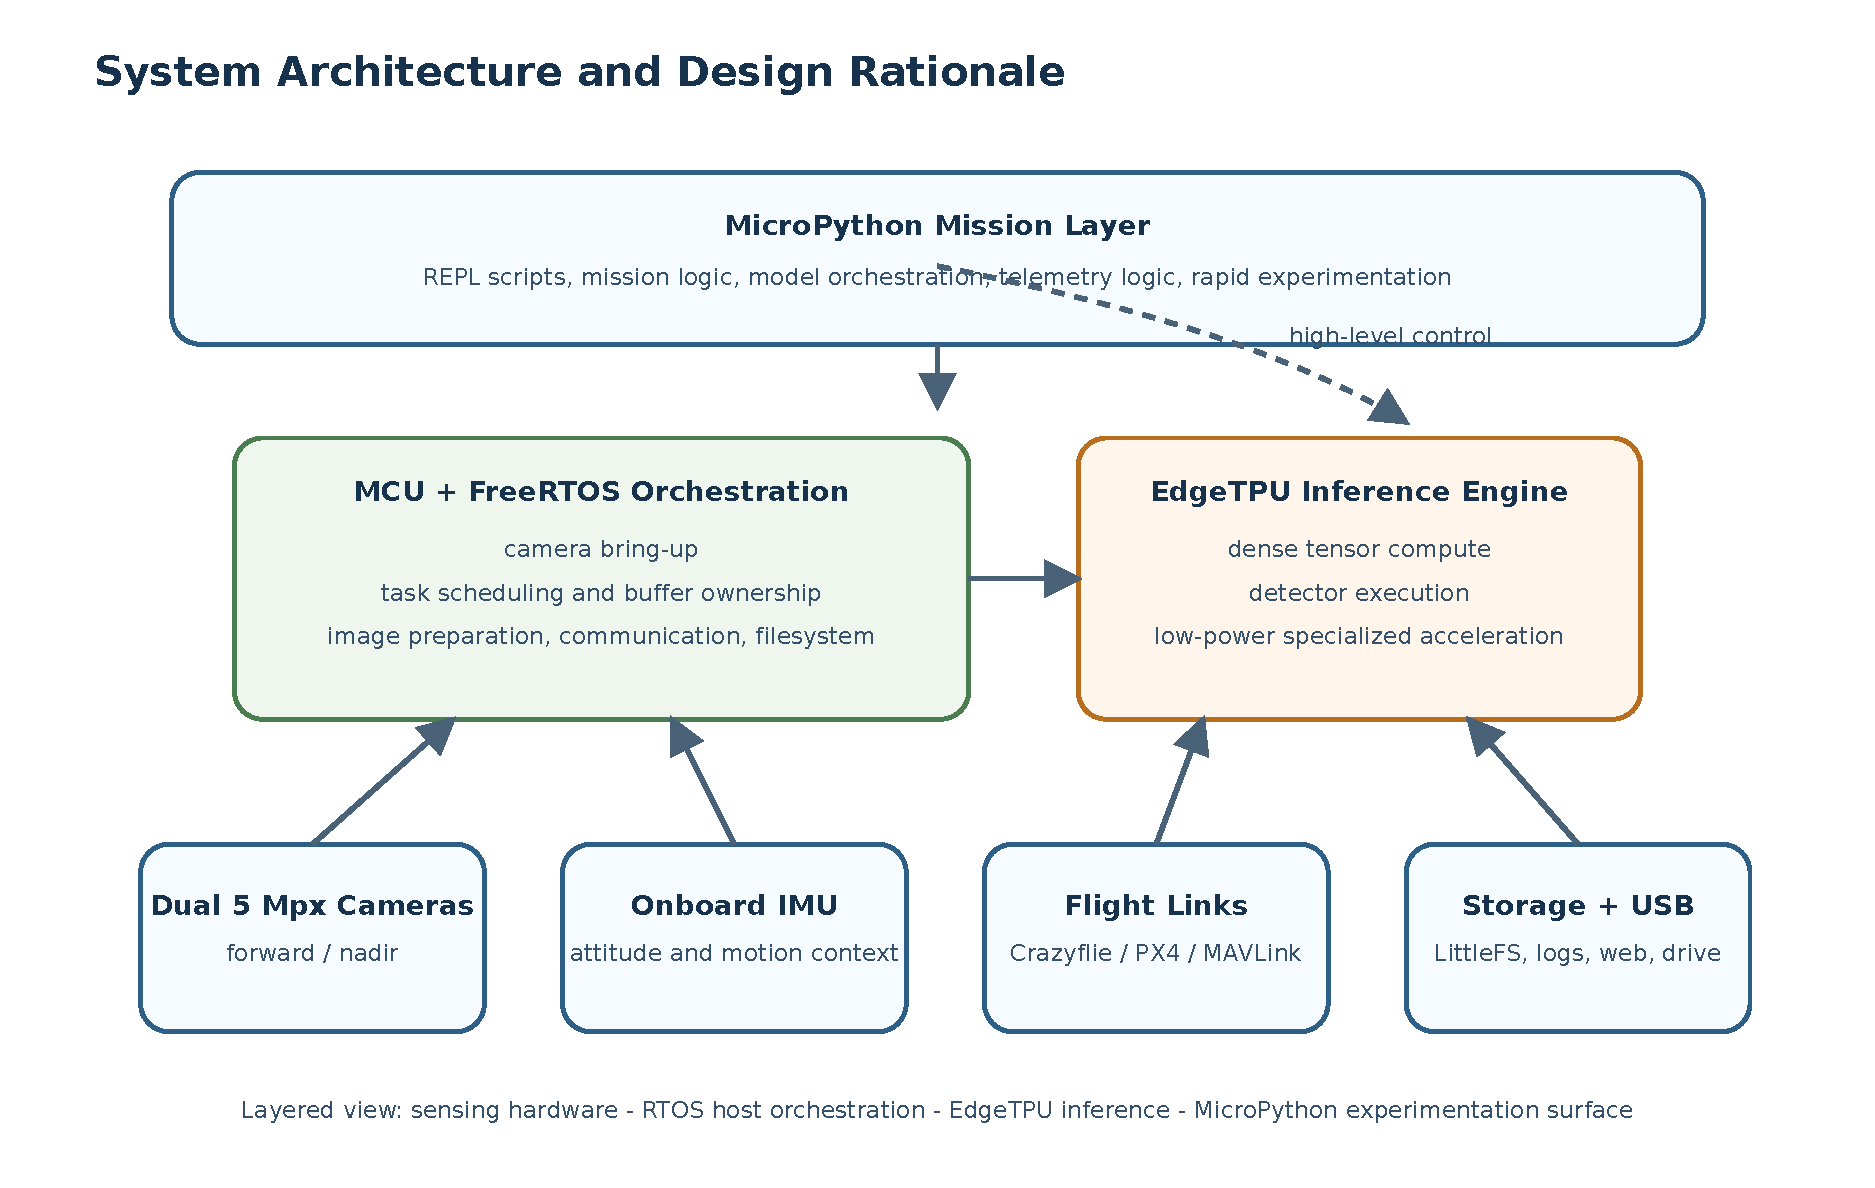
\includegraphics[width=0.94\textwidth]{figures/implementation_01_system_architecture.pdf}
\caption{Block-level view of the SentAI system architecture, highlighting the split between sensing hardware, MCU orchestration, EdgeTPU inference, and the script-oriented MicroPython layer.\label{fig:impl01}}
\end{figure}
\input{paper_mdpi_impl01.tex}

\subsection{RTOS Integration, Memory Layout, and Accelerator Feeding}
Figure~\ref{fig:impl02} shows the runtime pipeline used to keep the accelerator fed, with explicit staging, task handoff, and memory placement.
\begin{figure}[H]
\centering
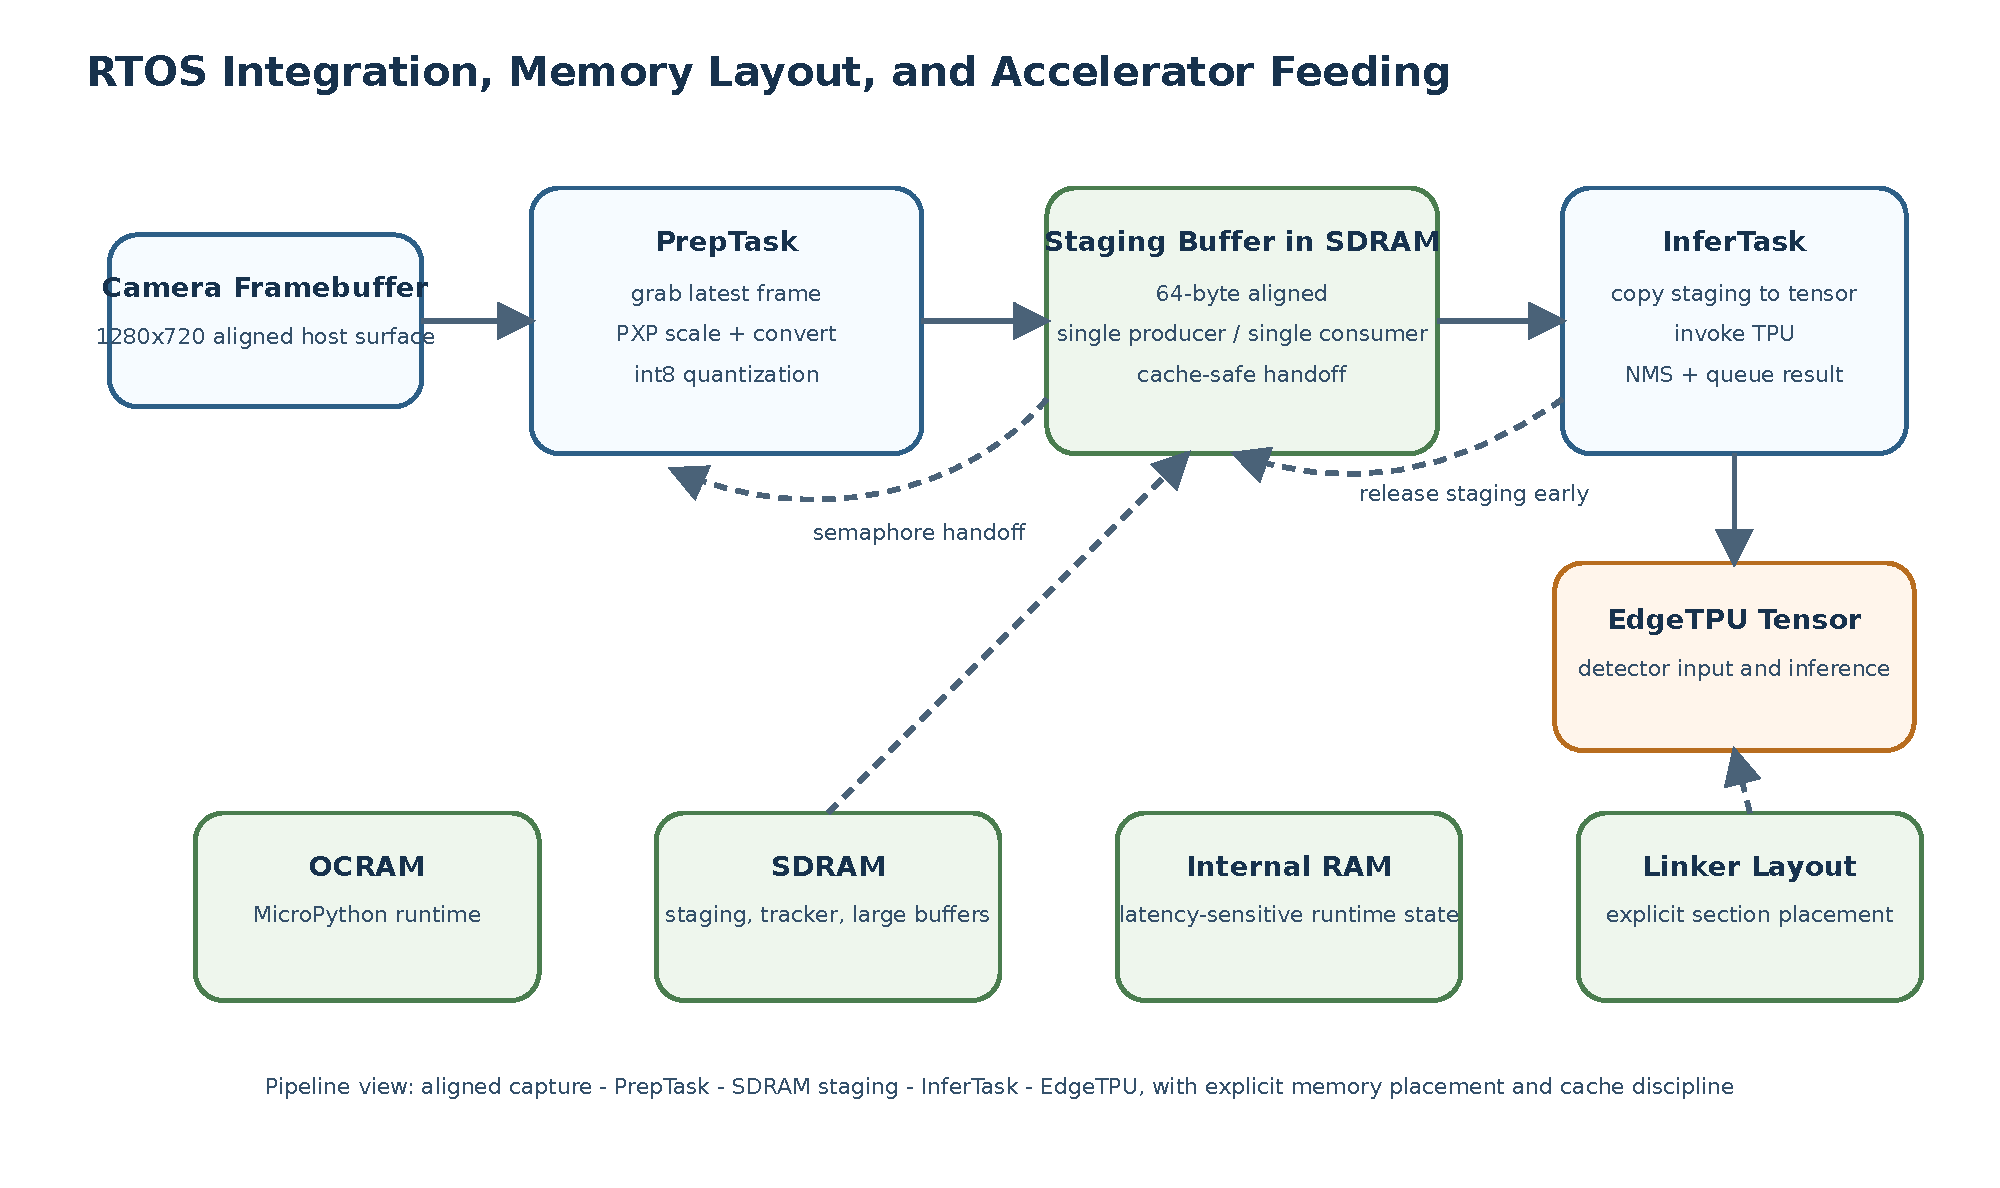
\includegraphics[width=0.98\textwidth]{figures/implementation_02_runtime_and_memory.pdf}
\caption{Block diagram of the RTOS and memory pipeline, showing aligned capture buffers, PrepTask, SDRAM staging, InferTask, and the EdgeTPU tensor path.\label{fig:impl02}}
\end{figure}
One of the main implementation claims of this work is that achieving
strong onboard vision performance on a compact MCU-plus-EdgeTPU platform
depends less on raw inference speed alone and more on how efficiently
the host prepares, places, and transfers data. This is particularly
visible in the code added relative to the initial fork, where the
runtime evolves from a board example into a carefully staged real-time
system.

The core execution environment is FreeRTOS. Rather than running
perception as a single sequential loop, the implementation decomposes
the workload into cooperating tasks with explicit ownership boundaries.
The most relevant example is the continuous detection pipeline, where
the code in \texttt{detection\_task.cc} organizes the system around a
preparation task and an inference task. The preparation task acquires
the latest frame, scales and converts it through the hardware pixel
pipeline, applies quantization when needed, and writes the result into a
staging buffer. The inference task copies the prepared staging contents
into the EdgeTPU input tensor, releases the staging buffer immediately,
and then executes inference and post-processing while preparation for
the next frame can already proceed. This design is not simply an
optimization; it is the mechanism through which the implementation turns
limited memory and compute resources into sustained throughput.

An important low-level detail is that the runtime does not feed the
detector directly from the raw camera bus format. The active camera
configuration captures native 1280x720 frames into 64-byte-aligned
framebuffers with a 4-byte-per-pixel host representation. In practice,
the software treats these buffers as XRGB8888-like surfaces because this
layout is easier to move through CSI DMA, cache maintenance, and the
RT1176 pixel pipeline than a tightly packed 3-byte RGB tensor. This is
precisely where the PXP block becomes essential rather than optional: it
converts the aligned capture surface into RGB888 output at the detector
input size, eliminating expensive per-pixel software shuffles on the
Cortex-M7.

This organization also clarifies the broader software split introduced
in the architecture chapter. The lower implementation layer is
task-oriented in C++, meaning that concurrency is expressed directly
through FreeRTOS tasks, semaphores, queues, and explicit buffer handoff
between producer and consumer stages. By contrast, the upper user layer
remains script-oriented in MicroPython, where these same services are
invoked as high-level operations without exposing the user to the
internal synchronization structure. The runtime and memory subsystem is
precisely where this separation becomes most meaningful: scripts can
request model loading, camera capture, or continuous detection, but the
correctness and performance of those operations depend on the
task-oriented C++ layer maintaining deterministic ownership over memory,
timing, and accelerator access.

The use of double-buffered staging is especially important because it
enforces a clean ownership discipline between producer and consumer
stages. The staging buffer is written by the preparation side and read
by the inference side under semaphore-controlled handoff, while the TPU
tensor is written only when the staging contents are ready. This
minimizes race conditions, reduces needless synchronization complexity,
and preserves the ability to overlap work. In a larger system with
abundant memory, one could compensate for poor orchestration by brute
force. In the present implementation, orchestration is the only
realistic way to maintain high frame rate while preserving the low-power
character of the platform.

The same section of code also shows why byte alignment becomes a
first-order systems concern. The staging area in SDRAM is explicitly
aligned to cache boundaries, while the PXP conversion path performs
cache clean-and-invalidate operations before DMA writes and invalidation
after completion so that stale boundary lines do not overwrite fresh
image data. This is needed because the TFLite arena is not naturally
aligned to the same cache-line granularity as the DMA engine. Without
that discipline, a seemingly minor mismatch between 16-byte tensor
allocation and 32-byte cache-line behavior would produce intermittent
corruption exactly at the stage where the detector input is assembled.

The memory layout reflects the same philosophy. The linker script
introduces a deliberate partitioning across internal memory, OCRAM,
heap, SDRAM, and a dedicated region for camera-related traffic.
MicroPython is placed explicitly in OCRAM rather than in the most
latency-sensitive memory regions, while large buffers, tracker state,
and staging areas are pushed into SDRAM where capacity matters more than
absolute access latency. This is visible both in the custom linker
script and in the pervasive use of explicit section placement such as
\texttt{.sdram\_bss}. The implementation thus accepts that not all
memory is equal and uses the linker as part of the optimization strategy
rather than as a passive build artifact.

This memory strategy also explains a design choice that would otherwise
look surprising from a purely model-centric viewpoint: the system first
tolerates a larger, alignment-friendly framebuffer representation and
only later collapses it into the compact RGB tensor expected by the
model. In other words, the runtime pays for structure before it pays for
compactness. That tradeoff is justified because aligned DMA and
deterministic hardware conversion are cheaper on this platform than
repeatedly manipulating tightly packed pixels in software.

This issue becomes more acute once YOLO-class detectors are considered.
Larger detector inputs significantly increase the pressure on staging
buffers, copied tensors, post-processing data, and runtime metadata. In
a conventional desktop pipeline this is almost invisible. On an MCU
platform it becomes decisive. The code therefore embodies a
memory-rearrangement strategy aimed at fitting the MicroPython runtime,
the real-time tasks, the tracker structures, and the camera-to-TPU
pipeline into a workable whole while minimizing inefficient copies. This
is one of the places where the implementation differs most strongly from
a conceptual prototype: the problem is no longer simply to run a model,
but to run it without collapsing the rest of the system.

The same logic informs the build system. The custom CMake configuration
aggregates a full embedded MicroPython build, nanopb-generated protocol
code, additional audio and communication components, and the custom
runtime sources into a single executable with a purpose-built linker
script. This makes the firmware itself part of the experimental method.
The implementation is not a loose collection of demos, but a
custom-built runtime whose compilation model, memory map, and
dependencies are aligned with the targeted deployment conditions.

From a research perspective, this subsection supports a broader claim:
on compact embedded AI platforms, the practical efficiency of a
specialized accelerator depends on the host system's ability to keep the
accelerator supplied with valid input at the right pace. The
implementation therefore treats memory organization and RTOS scheduling
as intrinsic parts of accelerator utilization rather than as secondary
engineering details.


\subsection{Dual-Camera Vision Pipeline and Perception Stack}
Figure~\ref{fig:impl03} illustrates how the two cameras, preprocessing path, detector, tracker, and geometry-aware projection stages interact inside the perception stack.
\begin{figure}[H]
\centering
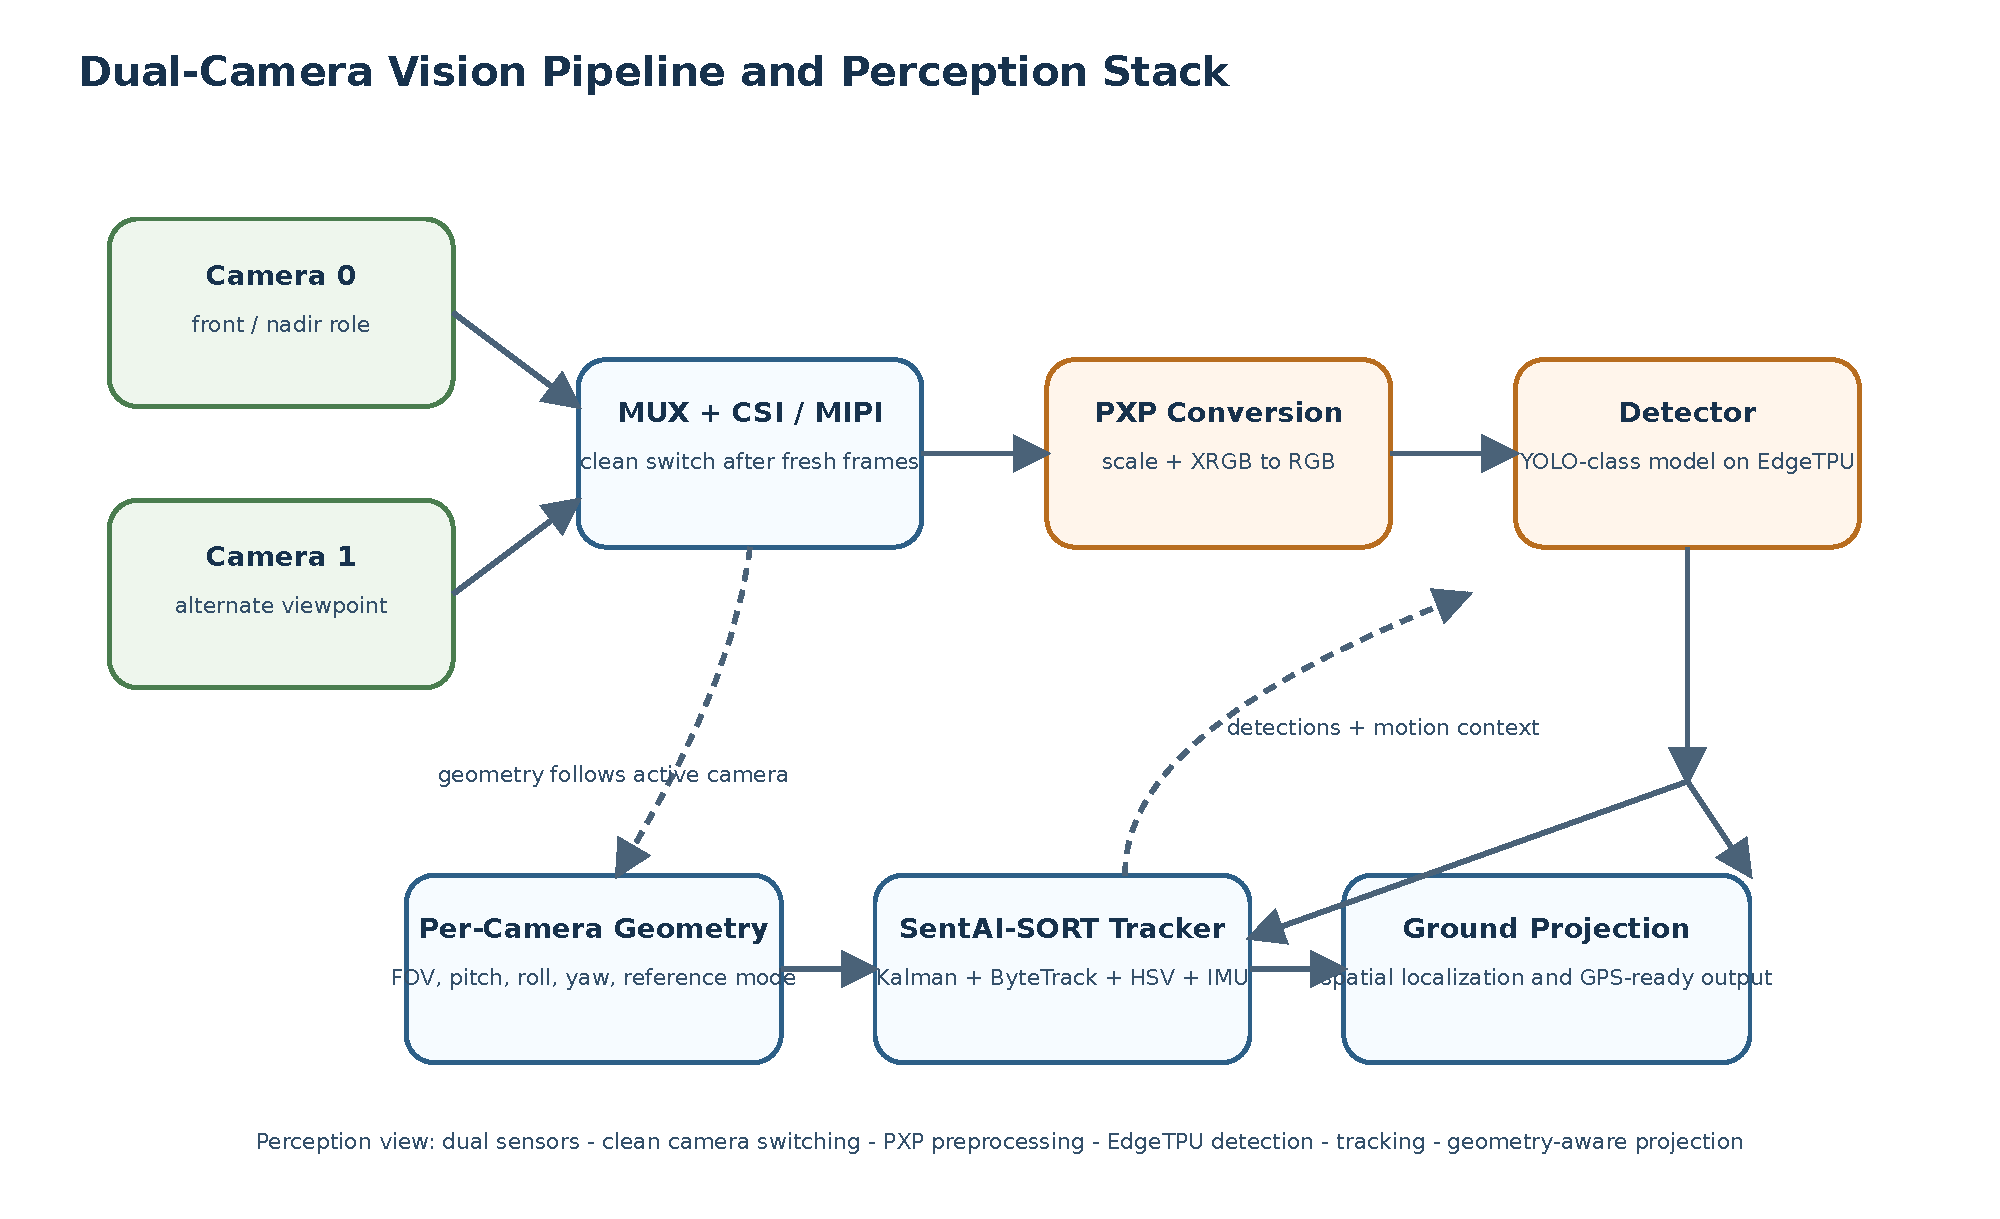
\includegraphics[width=0.98\textwidth]{figures/implementation_03_vision_pipeline.pdf}
\caption{Dual-camera perception pipeline with camera switching, PXP preprocessing, EdgeTPU detection, tracking, and ground-aware projection.\label{fig:impl03}}
\end{figure}
The perception implementation is built around the idea that high-quality
airborne vision is constrained as much by sensing geometry and data
movement as by the neural model itself. For this reason, the codebase
extends the original single-board camera model into a dual-camera system
with explicit support for runtime switching, per-camera geometry, and
high-resolution acquisition.

At the capture level, the cameras are integrated through the processor
camera subsystem and the MIPI CSI-2 path. This is an important
architectural choice because it prevents the image path from becoming
dominated by the kind of software-managed peripheral transfer overhead
that would be unacceptable for sustained real-time inference. The camera
stack is designed so that CSI and MIPI remain active even during
switching, which reduces disruption and helps preserve throughput. In
practical terms, the runtime exposes \texttt{sentai.camera.switch(id)}
while internally snapshotting the frame sequence and waiting until
enough fresh frames have arrived from the newly selected sensor to
guarantee a clean image. This is a small but important example of the
thesis that real embedded autonomy depends on disciplined treatment of
edge cases that benchmark-oriented prototypes often ignore.

The OV5640 integration itself is more substantial than a generic sensor
bring-up. Register control is handled over SCCB through the board I2C
interfaces, including model-ID verification, reset and power-down
sequencing, per-camera mirror and rotation adjustments, and
sensor-specific initialization on each side of the camera multiplexer.
On the video side, the datasheet-level interface still matters to the
architecture: the sensor family supports compact formats such as 8-bit
RGB565, but the host capture path on the RT1176 is engineered around
aligned 32-bit framebuffers and DMA-friendly pitches. As a result, the
implementation deliberately separates transport format concerns from
model-input format concerns instead of assuming that the detector can
consume the capture representation directly.

The implementation also recognizes that switching cameras is not useful
unless geometry travels with the switch. The perception pipeline
therefore maintains per-camera configuration for field of view, mount
pitch, mount roll, mount yaw, and ground-reference mode. This allows the
same runtime to support parallel cameras, perpendicular camera
placement, nadir sensing, or oblique views without hard-coding
assumptions about the sensor pose. In aerial robotics this is essential
because the operational meaning of a detection depends on how the camera
is mounted, not only on where the pixels appear.

The neural perception path itself is intentionally deployment-aware.
Frames are captured at the sensor side, then scaled and converted
through the hardware pixel pipeline before being prepared for the model
input tensor. This means the system can begin from richer camera
imagery, including workflows derived from native 1280-wide sensing,
while still feeding smaller quantized tensors to the detector. Such a
path is crucial for compact YOLO-family models, which often live in
tension between the need for more spatial detail and the strict memory
limits of MCU deployment.

One fine but important engineering point is that the PXP stage is not
used only for resizing. The camera receiver exposes raw host buffers
whose layout is convenient for aligned capture, cache maintenance, and
bus transfer, but not for direct detector input. The runtime therefore
uses PXP to transform XRGB-style capture surfaces into packed RGB output
with the exact detector dimensions, and then quantizes in place if the
TPU model expects int8 input. This avoids repeated software byte
shuffling, avoids ambiguities caused by aligned scanline storage, and
turns pixel-format conversion into a deterministic hardware stage of the
pipeline.

Above the detector, the implementation adds a custom tracking layer
referred to in code as SentAI-SORT. The design borrows the logic of
modern tracking-by-detection systems while adapting it to the realities
of a Cortex-M7-class host. The tracker combines an 8-state Kalman
formulation, a ByteTrack-style two-stage association process, and
compact HSV histogram features. Instead of relying on expensive
feature-based motion compensation, it uses IMU-informed compensation
derived from camera motion. This substitution is not only
computationally cheaper, but also better aligned with the sensing
resources already present on the platform.

The tracker is further extended with ground-plane projection and
optional GPS-referenced localization. Once altitude, heading, IMU
attitude, and camera geometry are known, detections can be mapped beyond
image coordinates into a spatial frame meaningful for the drone and for
downstream consumers. This is particularly important when the runtime is
used not only to detect objects, but also to generate position-aware
telemetry or to feed higher-level navigation policies.

The implementation therefore supports a wider claim than simple onboard
detection. It demonstrates that a small embedded AI platform can host a
complete airborne perception chain: dual high-resolution sensing,
viewpoint switching, quantized detection, lightweight tracking, motion
compensation, and spatial projection. In combination with model
switching, this also creates the conditions for multi-model operation in
which different detectors or visual policies can be applied according to
mission phase, camera viewpoint, or scene constraints.

Finally, the perception stack is complemented conceptually by the custom
YOLO model and the synthetic open dataset discussed elsewhere in the
paper. Although those assets are external to the code implementation,
they are consistent with the implementation logic described here: the
runtime is engineered so that compact detection models trained for nadir
and oblique drone views can be loaded dynamically and used as part of a
practical onboard autonomy workflow.


\subsection{Flight Control, Telemetry, and External Integration}
Figure~\ref{fig:impl04} summarizes the dual-target control model, in which one runtime connects local perception to both Crazyflie and PX4/MAVLink-centered workflows.
\begin{figure}[H]
\centering
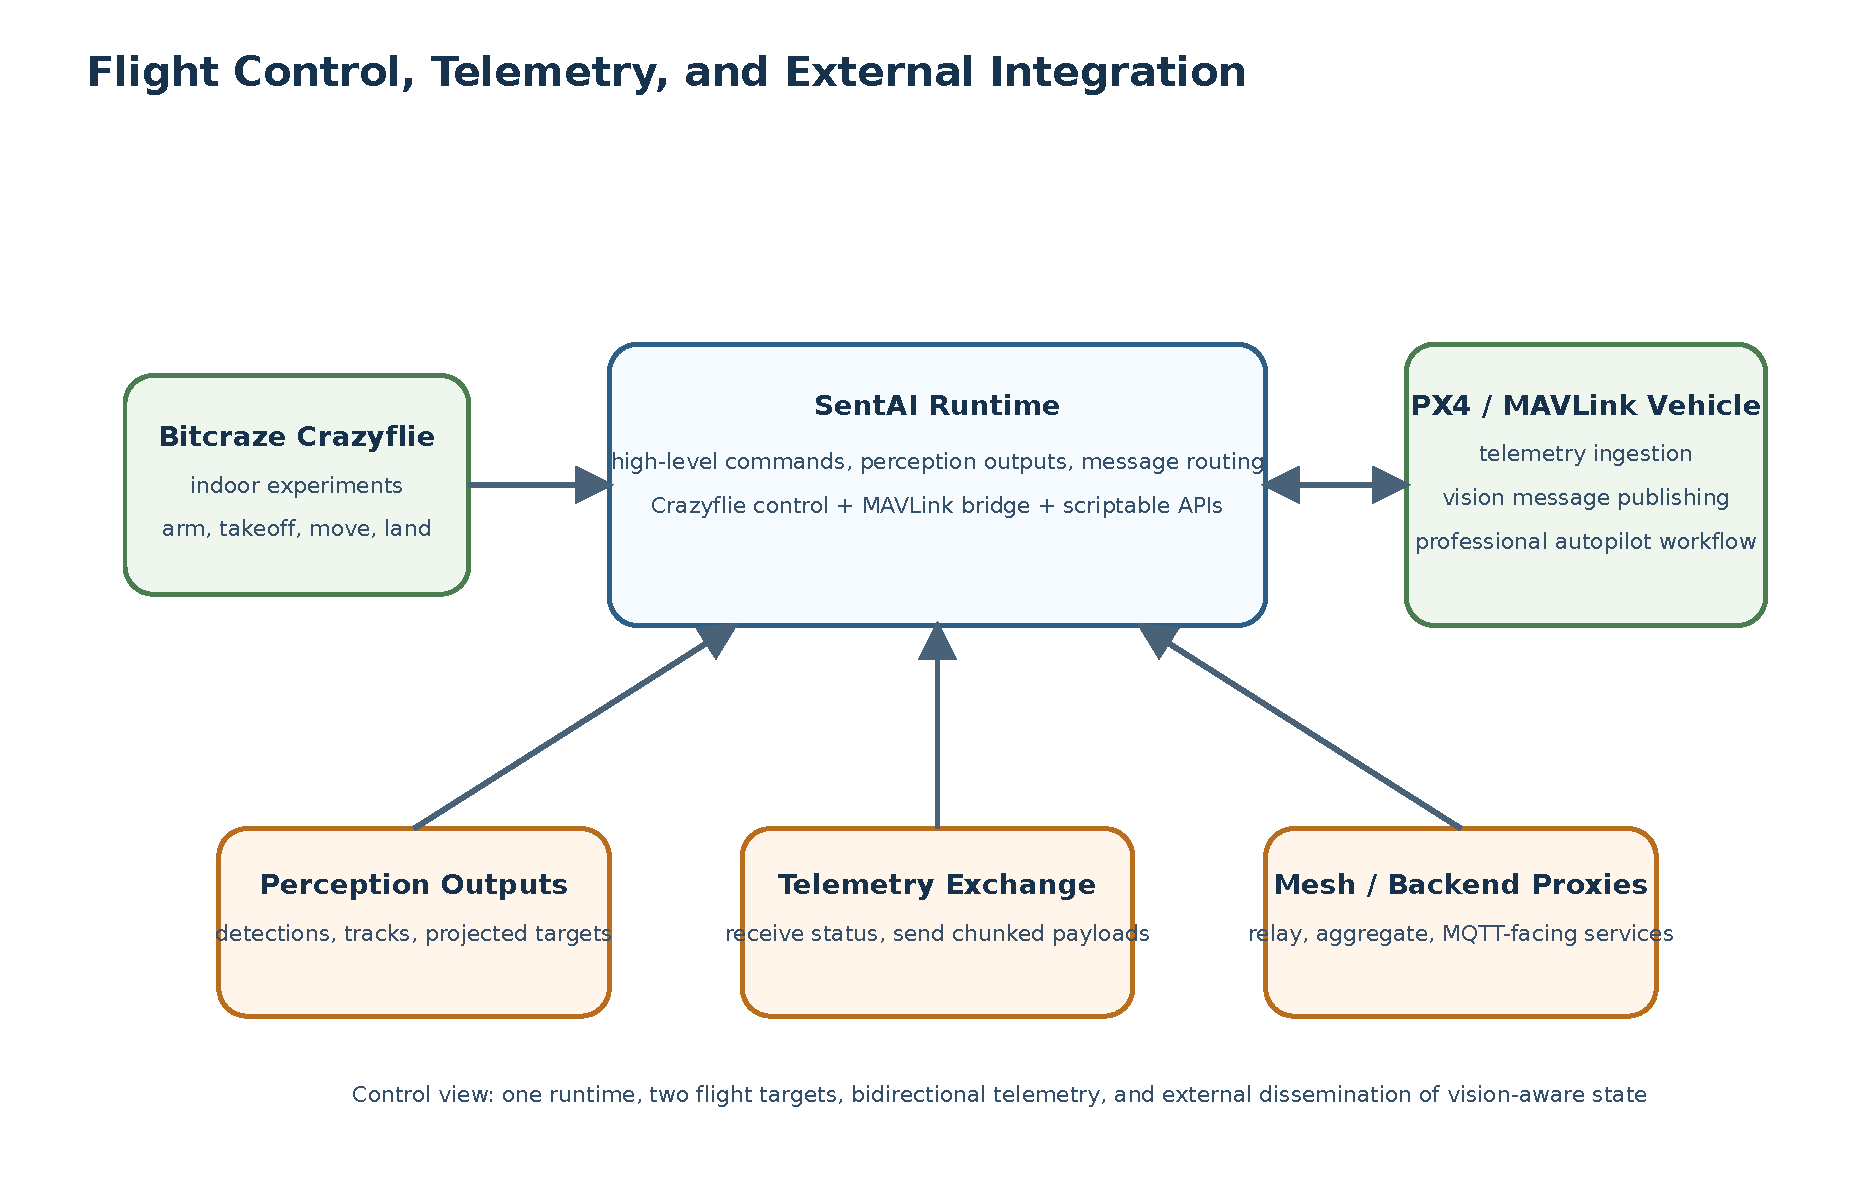
\includegraphics[width=0.94\textwidth]{figures/implementation_04_flight_and_telemetry.pdf}
\caption{Control and telemetry architecture spanning Crazyflie experimentation, MAVLink interoperability, and external backend dissemination.\label{fig:impl04}}
\end{figure}
The implementation does not stop at perception. A central design goal is
to make perception actionable in flight-relevant terms, and this is why
the runtime introduces two distinct but complementary control paths: one
centered on Bitcraze Crazyflie for indoor experimentation and one
centered on PX4-compatible communication through MAVLink for a more
standard professional autopilot ecosystem.

The Crazyflie path is valuable because it gives the research platform an
immediately usable indoor drone target that is lightweight, inexpensive,
and safe to iterate on in constrained spaces. In implementation terms,
the runtime exposes high-level flight functions for arming, takeoff,
landing, attitude control, hover-like motion, waypoint movement, and
basic link validation. The significance of this layer is less in the
underlying protocol details and more in the abstraction boundary it
creates: the experimental logic written in MicroPython can command a
real flying platform without descending into firmware-specific
implementation code for every new experiment.

The MAVLink path plays a different role. It positions the same
perception and scripting environment toward a standard autopilot
workflow, enabling connection to ground-control software and to a
PX4-style vehicle architecture. In the implementation, the MAVLink
bridge is built around the official message library and a dedicated
receive task, with queue-based delivery of decoded telemetry into the
runtime. This allows the platform to consume motion, position, and
status telemetry while also publishing onboard detections and system
messages back to the wider vehicle ecosystem. The result is a credible
bridge between a compact onboard perception unit and a more conventional
autopilot stack.

This bridge is not limited to a single control primitive. The runtime
exposes both transmission and reception semantics at the scripting
layer, including reception of autopilot telemetry and chunked
transmission of vision payloads that would not fit cleanly into a single
small embedded message. That detail matters because it shows the design
is meant for sustained exchange between perception and flight software
rather than for one-shot demo messages.

This dual-target approach is important conceptually. Many embedded AI
demonstrators either remain tied to a single experimental robot or aim
immediately at a professional stack without a low-risk iteration
platform. Here, the implementation supports both modes. Crazyflie serves
as a rapid prototyping platform for indoor validation, while MAVLink
provides compatibility with broader drone workflows. From a research
standpoint, this strengthens the portability of the proposed autonomy
layer.

The communication stack extends further through mesh and backend
services. The firmware side includes a compact binary vision message
protocol and bridges for wireless dissemination, while the repository
also adds backend proxy services that relay, aggregate, and expose
telemetry through ground-side interfaces such as MQTT. This is
significant because it shows that the implementation is intended to
operate as part of a distributed autonomy pipeline rather than as an
isolated board demo. Detections are not merely computed; they are
structured, transported, and made available to external systems.

In implementation terms, the control and communication layers provide
the missing operational dimension of embedded perception. A detector
running locally is useful only to a point. A detector that can feed a
Crazyflie experiment, inform a MAVLink autopilot context, publish
compact messages to external services, and remain scriptable from a
high-level runtime becomes much more valuable as a research instrument.
This is the level at which the runtime begins to resemble a true onboard
autonomy substrate rather than a perception benchmark harness.


\subsection{Programming Model and User-Facing Runtime Surface}
Figure~\ref{fig:impl05} provides a compact view of the user-facing runtime model, including the three USB access paths and the main groups of the \texttt{sentai} namespace.
\begin{figure}[H]
\centering
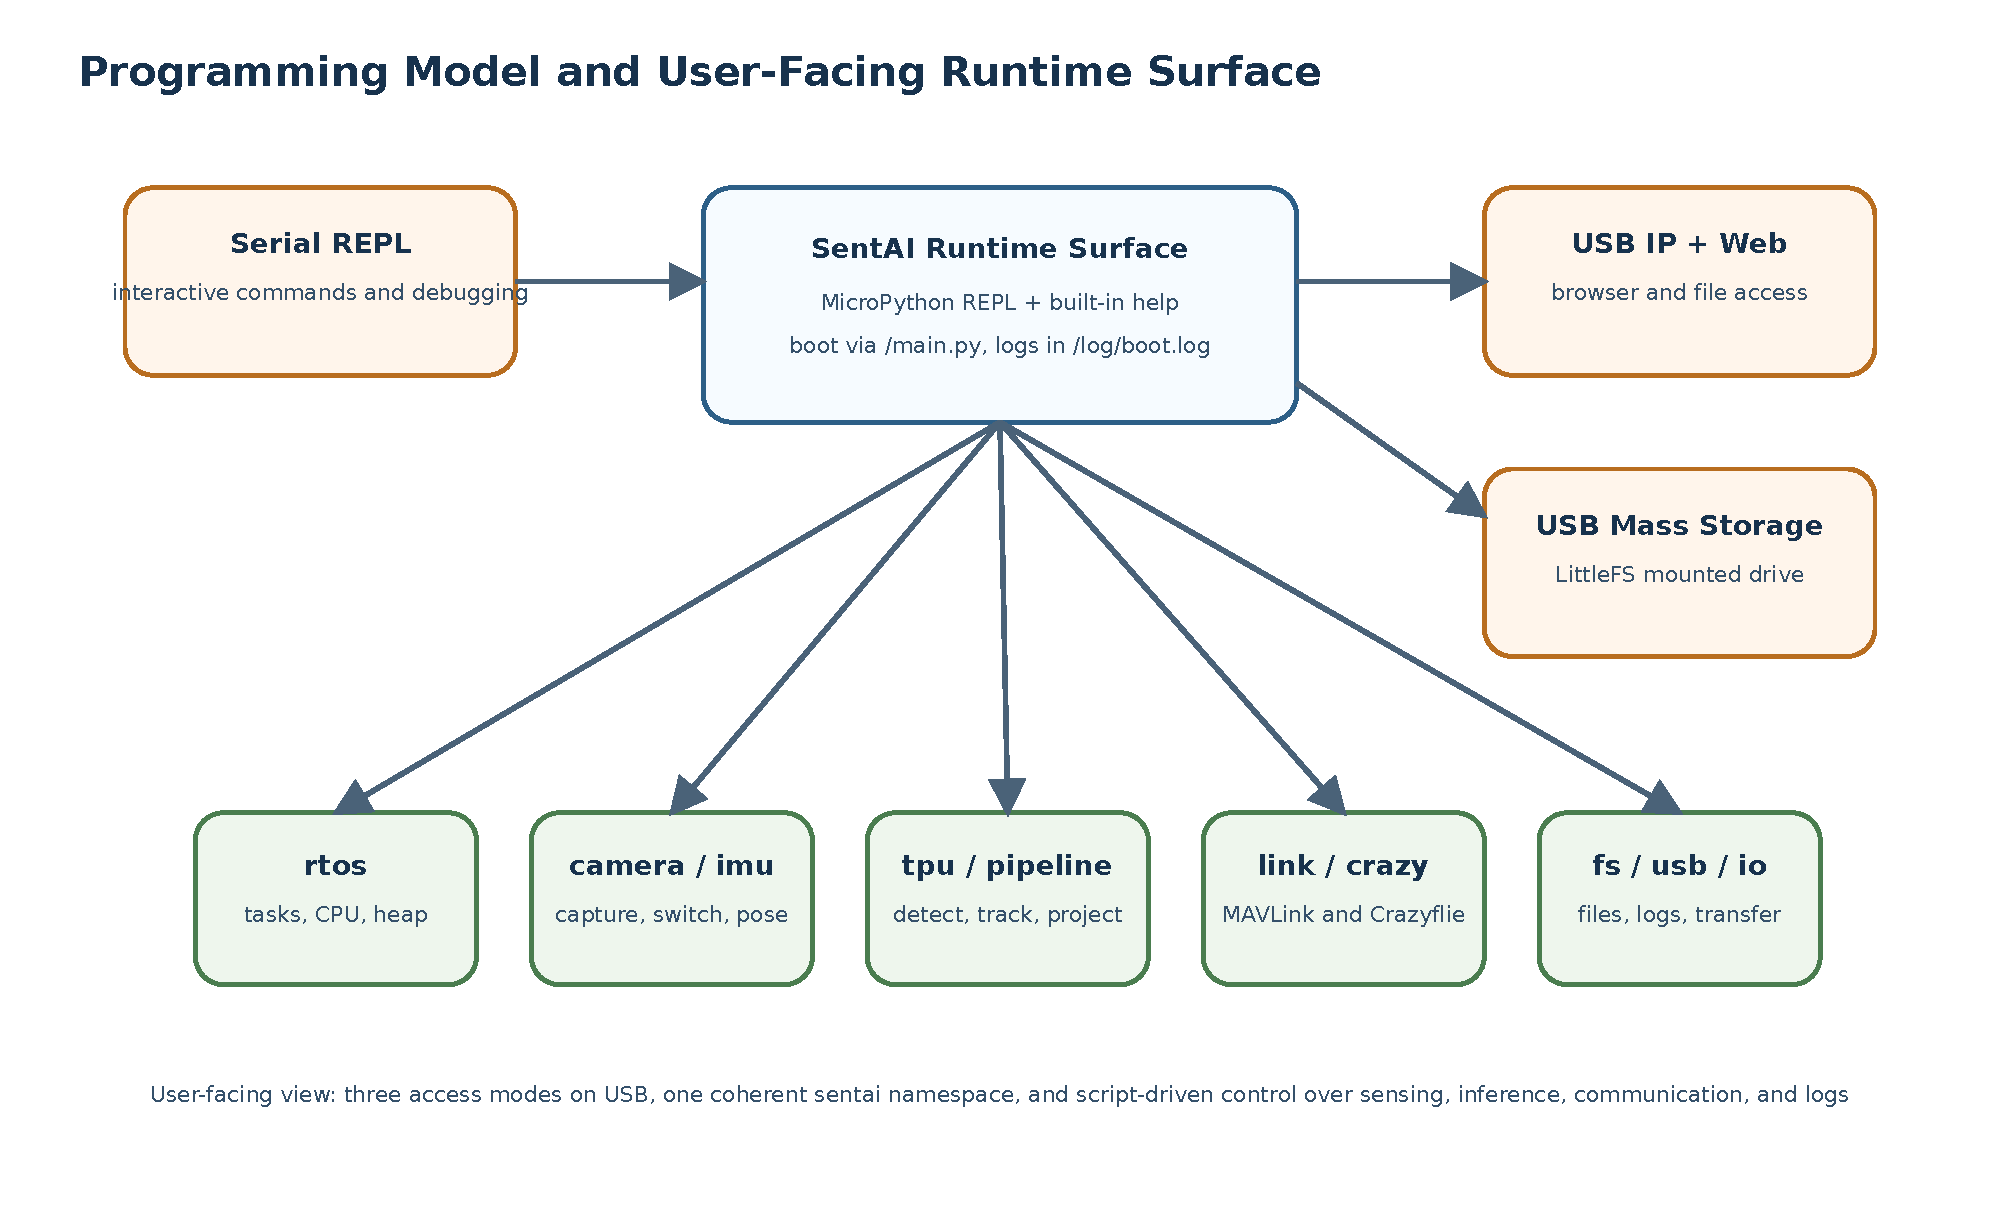
\includegraphics[width=0.98\textwidth]{figures/implementation_05_programming_model.pdf}
\caption{Programming model view showing REPL-centered access, USB service modes, boot artifacts, and the main runtime modules exposed through the \texttt{sentai} namespace.\label{fig:impl05}}
\end{figure}
An implementation of this kind must be evaluated not only by its
internal efficiency but also by how coherently it exposes its
capabilities to the user. This is especially important on MCU-based
platforms, where debugging is often more difficult than on Linux-class
systems because the developer has less runtime introspection, fewer
interactive tools, and a much narrower margin for trial-and-error when
something goes wrong during boot or during a real-time task interaction.
For this reason, SentAI does not expose a single debugging path, but a
small set of complementary connection modes over USB that make the board
significantly easier to inspect and operate in practice.

The first mode is an interactive MicroPython REPL available over the
serial interface, which allows a researcher or operator to connect
directly to the board, inspect the runtime state, execute commands live,
load scripts, and request contextual help from within the system itself.
This is a consequential design choice: the platform is not only flashed
and executed as a fixed firmware image, but can also be interrogated and
steered interactively during development and testing. In practice, the
REPL becomes the primary entry point for experimentation, rapid
diagnosis, and iterative mission design.

The second mode is USB networking over IP, through which the firmware
exposes an onboard web server and file-browser interface. This gives the
board a lightweight service surface that can be reached directly from
the host, making it possible to inspect and transfer artifacts without
depending exclusively on the serial console. The third mode is USB mass
storage, in which the LittleFS user partition is exposed as a mounted
drive so that images, scripts, and models can be uploaded or downloaded
directly from the host machine. Taken together, these three USB-facing
paths, namely serial REPL, IP connectivity with web access, and mounted
LittleFS storage, form a practical answer to the usual debugging and
deployment friction of MCU-based systems.

The built-in help interface available from the REPL makes this
programming model discoverable without forcing the user to leave the
target system. This matters because the runtime is relatively rich: it
does not expose a single detector call or a single flight command, but a
full namespace of platform primitives intended to support sensing,
inference, telemetry, storage, and high-level control from one embedded
environment. The same environment also supports script-driven startup
through \texttt{/main.py}, which is automatically executed at boot
before the interactive session begins. This gives the platform an
important dual character: it can behave as an interactive research
instrument during development, but it can also behave as a self-starting
embedded application once the desired mission logic has been written.

This startup behavior is complemented by a boot logging mechanism
implemented directly in the runtime. During initialization, console and
driver output are captured into \texttt{/log/boot.log}, while the
previous boot log is rotated to \texttt{/log/boot\_old.log}. This is an
important practical feature for embedded debugging, because many
failures on an MCU platform occur before a user can attach interactively
to the REPL. By preserving the initialization trace on LittleFS, the
system allows the user to inspect the outcome of FreeRTOS bring-up,
early peripheral initialization, and startup script execution even after
the board has already moved past the failing point.

The \texttt{sentai} namespace organizes the platform into functional
modules such as \texttt{io}, \texttt{rtos}, \texttt{tpu}, \texttt{fs},
\texttt{camera}, \texttt{imu}, \texttt{usb}, \texttt{link},
\texttt{crazy}, and \texttt{pipeline}, alongside several other utility
interfaces. This structure is significant because it reveals the
intended user abstraction: the operator is not expected to manipulate a
collection of unrelated firmware endpoints, but to work with a coherent
runtime in which device functions are grouped by task and by
experimental purpose. The platform can query RTOS state, inspect heap
usage, load models, capture or switch cameras, read inertial
measurements, start a continuous detector, track objects, communicate
over MAVLink, or command a drone, all through a single embedded language
environment.

This helps explain why MicroPython is a central implementation choice
rather than a peripheral convenience. The interpreter does not replace
the lower-level real-time system; instead, it defines a stable
experimentation layer above it. The help text demonstrates this duality
clearly. On one hand, users access simple operations such as
\texttt{sentai.camera.to\_tensor()} or \texttt{sentai.tpu.invoke()}. On
the other hand, the same interface reaches into advanced platform
features such as tracking events, per-camera geometry, ground-plane
projection, and MAVLink message exchange. The implementation thereby
condenses a complex firmware system into a form that is operable from
concise Python scripts.

Several modules are especially important for understanding the research
value of the platform. The \texttt{rtos} module exposes runtime
observability primitives such as task inspection, CPU statistics, and
heap information, which are essential when the system is tuned for
sustained real-time throughput. The \texttt{tpu} module provides the
basic inference control plane: model loading, tensor access, invocation,
quantization metadata, and detector-oriented post-processing. The
\texttt{camera} module complements it by managing capture, JPEG export,
transfer to the tensor path, runtime camera switching, and frame
sequencing. The \texttt{imu} module supplies the inertial measurements
needed by viewpoint-aware tracking and projection. The \texttt{fs} and
\texttt{usb} modules support a practical workflow in which models,
scripts, captured outputs, and debugging artifacts can be transferred to
and from the device without rebuilding the firmware for every iteration.

The help surface also shows that these capabilities were designed to be
exercised directly from the target rather than only through host-side
tooling. Typical examples include immediate tensor feeding from the
camera, live detector startup, autopilot connection, or direct Crazyflie
flight commands, for example:

\begin{Shaded}
\begin{Highlighting}[]
\NormalTok{sentai.camera.to\_tensor()}
\NormalTok{sentai.tpu.invoke()}
\BuiltInTok{print}\NormalTok{(sentai.tpu.detect())}
\end{Highlighting}
\end{Shaded}

\begin{Shaded}
\begin{Highlighting}[]
\NormalTok{sentai.link.init(}\DecValTok{57600}\NormalTok{)}
\NormalTok{sentai.pipeline.start(}\FloatTok{0.3}\NormalTok{, }\FloatTok{0.45}\NormalTok{, }\DecValTok{50}\NormalTok{, }\VariableTok{True}\NormalTok{)}
\ControlFlowTok{while} \VariableTok{True}\NormalTok{:}
\NormalTok{    msg }\OperatorTok{=}\NormalTok{ sentai.link.receive()}
    \ControlFlowTok{if}\NormalTok{ msg:}
        \BuiltInTok{print}\NormalTok{(msg)}
\end{Highlighting}
\end{Shaded}

\begin{Shaded}
\begin{Highlighting}[]
\NormalTok{sentai.crazy.init()}
\NormalTok{sentai.crazy.arm()}
\NormalTok{sentai.crazy.fly(}\FloatTok{0.3}\NormalTok{, }\DecValTok{3000}\NormalTok{)}
\NormalTok{sentai.crazy.fly\_stop()}
\end{Highlighting}
\end{Shaded}

At the control and autonomy layer, \texttt{link}, \texttt{crazy}, and
\texttt{pipeline} form the most distinctive part of the namespace. The
\texttt{link} module exposes MAVLink communication as a first-class
runtime capability, allowing the board to exchange telemetry and
structured messages with an autopilot or a ground-control system. The
\texttt{crazy} module does the same for the indoor Crazyflie target,
exposing high-level flight functions directly to Python. The
\texttt{pipeline} module unifies the continuous detector, tracker, event
stream, per-camera geometry, and pose-aware projection logic into a
single interface. Together, these modules reveal the real ambition of
the implementation: the embedded AI platform is not only an inference
endpoint, but a scriptable autonomy substrate in which perception,
communication, and high-level flight behavior can be composed
interactively.

The \texttt{pipeline} module is especially illustrative. According to
the documented runtime surface, it exposes continuous detection,
statistics, tracker snapshots, event streams, configurable association
parameters, pose setting, and per-camera geometry. This is not a trivial
wrapper around a detector. It is the public face of the deeper
implementation presented in the previous subsections: the parallel
camera-to-TPU pipeline, the tracking-by-detection logic, and the
geometry-aware projection model all become accessible through a minimal
but expressive Python API. The same can be said for the \texttt{link}
and \texttt{crazy} modules, which reveal that flight and telemetry
functions are not separate applications but first-class capabilities of
the runtime itself.

From a research-methodology perspective, this matters because it changes
the pace and style of experimentation. A researcher can move from
firmware bring-up to mission logic, data capture, tracking inspection,
and communication testing without leaving the same runtime environment.
This reduces iteration cost and makes the platform more suitable for
exploratory autonomy research, where control policies, perception
thresholds, and communication strategies change frequently.

The built-in help surface also provides indirect evidence of
implementation maturity. A platform that documents precise operational
behaviors, module boundaries, argument conventions, and example
workflows has generally progressed beyond proof-of-concept code. In
SentAI, the fact that these capabilities can be explored directly from
the serial REPL supports the claim that the implementation has been
organized as a reusable experimental environment rather than as a
collection of hidden firmware entry points.

The programming model therefore completes the overall argument of the
chapter. The EdgeTPU provides the inference power, the MCU and RTOS
provide the orchestration, the cameras and IMU provide the sensing
context, and MicroPython makes the whole system operable as a research
platform. The implementation succeeds not only when it runs efficiently,
but when it turns that efficiency into a usable and extensible interface
for autonomous drone experimentation.


\section{Discussion}
This chapter describes the implementation of SentAI as a research
platform positioned at the intersection of embedded AI acceleration,
real-time systems, and autonomous drone control. The central thesis of
the implementation is that an EdgeTPU-class accelerator is
simultaneously low-power and computationally powerful enough to justify
a much tighter integration with an MCU than is common in larger
companion-computer architectures. Rather than treating the accelerator
as a peripheral attached to a heavy host, the design treats the MCU and
EdgeTPU as a compact co-processing pair: the MCU handles sensing,
scheduling, memory orchestration, communication, and high-level control,
while the EdgeTPU is driven as the main execution substrate for neural
inference.

An equally important framing point is that the implementation starts
from an open-source platform with significant unrealized potential and
deliberately pushes it toward industrialization. In other words, the
work is not only about extending Coral Micro with additional
capabilities, but about transforming an accessible open-source base into
a system that exhibits more production-oriented behavior: higher
sustained throughput, better control of memory and latency, richer
sensor integration, clearer runtime abstractions, and a software
structure that can support repeated deployment rather than isolated
demonstrations.

The implementation presented in this work differs substantially from the
initial fork baseline by transforming a board-oriented demo environment
into a programmable autonomous-flight runtime. The main engineering
question is not only whether inference can run onboard, but how to
maximize accelerator utilization, sustain real-time responsiveness, and
preserve a lightweight and low-power hardware profile suitable for
micro-UAV operation. This leads to a design in which memory placement,
transfer scheduling, camera integration, scripting boundaries, and
telemetry abstractions become first-order implementation concerns. In
this sense, the chapter documents a move from open-source
proof-of-potential to an embedded system engineered with
production-performance objectives in mind.

The chapter is organized into the following subchapters:

\begin{enumerate}
\def\labelenumi{\arabic{enumi}.}
\tightlist
\item
  \url{implementation_01_system_architecture.md}, which explains the
  hardware-software co-design and the motivation for pairing an MCU with
  an EdgeTPU on a lightweight drone-oriented board.
\item
  \url{implementation_02_runtime_and_memory.md}, which analyzes the RTOS
  integration, linker-level memory layout, staging buffers, and the
  host-side logic required to keep the accelerator fed efficiently.
\item
  \url{implementation_03_vision_pipeline.md}, which details the
  dual-camera subsystem, the real-time image path, tracking, projection,
  and the deployment of YOLO-class detectors.
\item
  \url{implementation_04_flight_and_telemetry.md}, which presents the
  dual-target control strategy spanning Crazyflie and PX4/MAVLink,
  together with telemetry and backend integration.
\item
  \url{implementation_05_programming_model.md}, which studies the
  MicroPython layer and uses the platform help system as evidence of how
  the embedded capabilities are exposed as a coherent experimental
  interface.
\end{enumerate}

Taken together, these sections argue that the implementation is best
understood as an exercise in practical embedded-AI industrialization:
the work does not merely deploy neural inference on a small board, but
systematically resolves the hardware and software bottlenecks that arise
when such inference must coexist with flight control, camera switching,
runtime programmability, and constrained memory resources. The overall
contribution is therefore to show how an open-source platform can be
matured toward a more production-capable embedded autonomy stack without
abandoning its accessibility, compactness, or low-power design
philosophy.


\section{Conclusions}
\emph{The quantitative headline summary is in \url{evaluation.md} §7,
Table 7. The narrative below is the systems-integration framing of what
those numbers mean.}

This work presented an effort to turn a lightweight open-source embedded
AI board into an open inference and autonomy platform for drones. The
central result is that an EdgeTPU-class accelerator can be paired
effectively with an MCU when the surrounding software stack is designed
to keep sensing, memory movement, scheduling, telemetry, and
programmability aligned. The goal is not to imitate a Linux-class
companion computer, but to show that a much lighter board can still
support meaningful onboard inference and autonomy when the system is
treated as a co-design problem rather than as a loose collection of
features.

The implementation extends the original Coral Micro board from which the
design started with a number of capabilities required for autonomous
drone research: a full MicroPython runtime, dual 5 Mpx cameras, onboard
IMU integration, a parallel camera-to-EdgeTPU perception pipeline,
CPU-side TensorFlow Lite Micro inference, lightweight tracking and
projection, runtime camera and model switching, interactive debugging
and deployment paths, obstacle-map reporting for PX4-style collision
prevention, dual-target control support spanning both Bitcraze Crazyflie
and PX4/MAVLink-style workflows, and an integrated set of classical ML
primitives that can be invoked directly from scripts. Taken together,
these additions define our MCU-EdgeTPU board as a more complete embedded
inference environment.

One of the clearest conclusions is that the hardest problems in compact
airborne AI systems often sit outside the neural model. Much of the
implementation effort went into ensuring that images could be acquired,
transferred, staged, quantized, and scheduled in real time without
breaking the low-power and low-mass profile of the platform. Host-side
systems engineering, especially memory placement, ownership discipline,
boot-time observability, and developer-facing tooling, proved just as
important as the accelerator.

The platform also contributes a broader methodological point. By
combining a task-oriented C++ runtime with a script-oriented MicroPython
layer, the system shows that it is possible to preserve real-time
discipline while still exposing an interface suitable for rapid
experimentation. This is particularly valuable in drone autonomy, where
sensing configuration, communication policies, flight behaviors, and
even the choice between accelerator-backed and MCU-only models are
rarely fixed early in development. The ability to move repeatedly
between low-level performance engineering and high-level scripting is
one of the main reasons the resulting system is useful as a research
artifact. The same interface now supports a wider set of embedded ML
experiments, including clustering, anomaly scoring, sequence modeling,
reinforcement learning, and lightweight SLAM, which further supports the
view of the runtime as an environment for embedded inference workflows
rather than a narrow detector wrapper.

Finally, the work suggests that lightweight open-source embedded AI
boards should not be viewed only as educational or prototyping tools.
With sufficient attention to integration quality, memory engineering,
runtime design, and flight-stack interfaces, they can serve as
technically relevant foundations for more demanding autonomous systems.
The resulting platform stands both as a concrete implementation and as
an argument for taking accessible open hardware seriously as a basis for
embedded autonomy research.


\subsection{Future Work}
Several directions follow naturally from the present implementation. A
first line of future work concerns completing the symmetry between the
two flight targets. Although the platform already exposes both
Crazyflie-oriented and MAVLink-oriented control paths, a fuller
unification of mission abstractions, telemetry semantics, and safety
behaviors across both environments would strengthen the claim of a truly
portable high-level autonomy layer. This includes deeper integration
with PX4 control modes, more explicit offboard control patterns, richer
use of onboard obstacle maps inside autopilot workflows, and a cleaner
common contract between indoor experimental flights and more operational
autopilot-driven deployments.

On the perception side, future work should extend the current
multi-camera and multi-model logic toward tighter cross-camera
continuity. The present system supports runtime camera switching,
per-camera geometry, and viewpoint-aware projection, but does not yet
provide full track handoff across cameras. A next step would therefore
be to reproject existing track hypotheses across viewpoints and preserve
track identity when a target moves from one sensor to the other. This
would make the dual-camera architecture more than a switching mechanism
and turn it into a more integrated multi-view perception system.

A second major direction concerns model deployment. The current work
argues for compact YOLO-style detectors and open synthetic pre-training
assets, but there remains significant room for improvement in model
adaptation, quantization robustness, and scene-specific specialization.
Future work could evaluate alternative compact detectors, mixed-model
cascades, task-specific switching policies, and better domain adaptation
between synthetic and real aerial imagery. It would also be valuable to
formalize when workloads should remain on the EdgeTPU and when they
should fall back to CPU-side TensorFlow Lite Micro execution, especially
in missions that mix fast detection with lightweight auxiliary models.
In particular, the regulation-aware navigation framing introduced in
this work would benefit from models trained not only for general
detection, but also for explicit recognition of flight-relevant
constraints in inhabited spaces.

The expanded embedded-ML runtime opens a further line of work beyond
classical detector deployment. The current implementation already
exposes clustering, anomaly detection, sequence modeling, reinforcement
learning, and lightweight SLAM primitives, but these remain building
blocks rather than a mature learning framework. Future work could
evaluate how these modules interact in closed-loop autonomy settings,
how they should share memory and telemetry channels with the perception
stack, and which of them are practically robust enough for long-duration
field experiments on an MCU-class platform.

Another important direction is deeper optimization of the memory and
dataflow path. The current implementation already uses task parallelism,
staging buffers, and explicit SDRAM placement, but more aggressive
zero-copy strategies, richer DMA-assisted transfer patterns, or
compiler-assisted layout optimization may further improve throughput and
energy efficiency. The same is true for the host-side interaction with
the EdgeTPU: a richer study of tensor residency, batching patterns, or
asynchronous execution opportunities could reveal additional performance
margins on this class of embedded platform.

The developer experience can also be extended. The current system
already provides a serial REPL, IP-based access with a web interface,
mounted LittleFS transfer, boot logging, and boot-time execution through
\texttt{main.py}. Future work could unify these into a more formal
device-management workflow with remote script deployment, structured
runtime tracing, automated collection of telemetry and images, artifact
export for both obstacle and vision messages, and reproducible
experiment packaging. Such tooling would be especially useful if the
platform is to be used by multiple researchers or integrated into longer
experimental campaigns.

At the system level, the project also opens a path toward broader
hardware generalization. One of the arguments made throughout this work
is that the EdgeTPU is a sufficiently capable low-power inference
primitive to justify close integration with an MCU. A natural next step
is therefore to explore how much of the present design can be ported to
other MCU families, other camera configurations, or future open-source
boards with similar accelerator-centric architectures. If successful,
this would strengthen the broader claim that lightweight
accelerator-plus-MCU designs are a viable class of embedded autonomy
platform rather than a single-board exception.

Taken together, these directions suggest that the present work is less
an endpoint than a foundation. The current implementation establishes
the runtime, sensing, memory, control, and experimentation abstractions
needed for a compact embedded autonomy stack. Future work can now build
on this base to improve viewpoint continuity, flight-platform symmetry,
regulation-aware perception, deployment tooling, embedded learning
workflows, and cross-platform generalization.


\end{document}